
On peut maintenant faire apprendre au réseau nimporte quelle application linéaire.
Par exemple la moyenne :

\begin{figure}[H]
    \center
    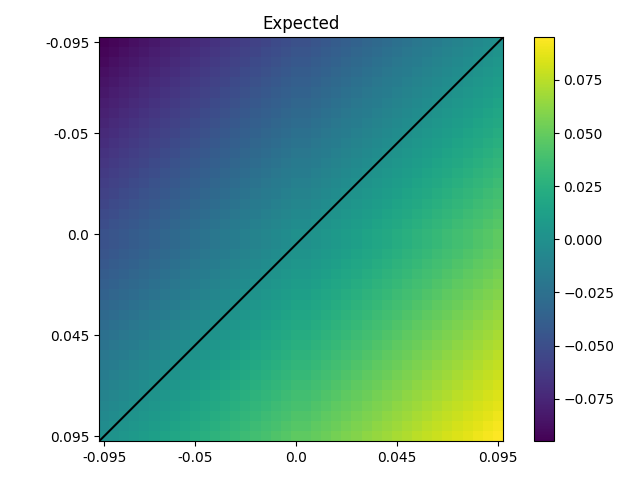
\includegraphics[height=\petit]{pict/moy/expected}
    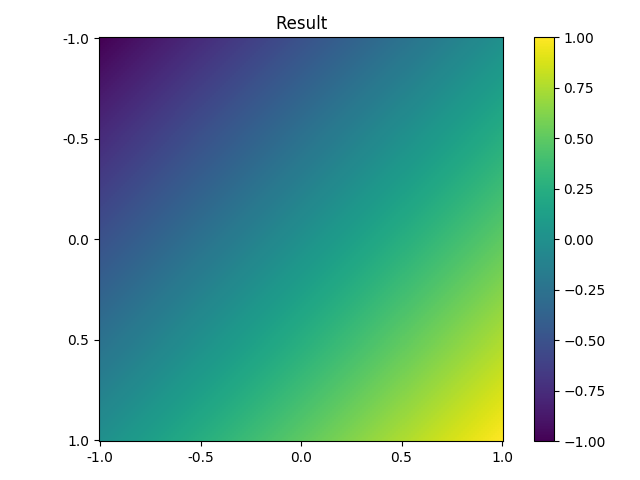
\includegraphics[height=\petit]{pict/moy/result}
	\caption{Apprentissage de la moyenne}
    \begin{center}
        \textit{
        A gauche, le résutltat atendu, a droite, celui renvoyé.\\
        $x_1$ en absice, $x_2$ en ordonées.
        }
    \end{center}
	\label{fig:moy}
\end{figure}
\vspace{-12pt}

On peut voir que la descente de gradients se fait a merveille.
Aucunes difference ne sont visibles : en effet les poids associés aux deux noeuds sont les suivants :
\begin{equation*}
    w_1 = 0.50000010
    \;\;\;\;\;\;\;\;\;
    w_2 = 0.50000024
\end{equation*}
On peut voir qu'aux aproximations processeur, les poids sont les bons pour faire la moyenne de deux nombres :
\begin{equation*}
    m =\frac{n_1 + n_2}{2} = 0.5 \times n_1 + 0.5 \times n_2
\end{equation*}
